\subsection{Rancangan Struktural}
\label{subsec:rancangan-struktural}

Arsitektur sistem yang akan dibangun akan digambarkan dengan Package Diagram. Sistem akan dibagi menjadi 3 kelompok komponen utama, yaitu eth2dgraph sebagai komponen luar sistem yang akan mengakses Ethereum Archive Node, komponen sistem utama yang terdiri dari DgraphDB dengan modul data access, Smart Contract Enricher, Vector Database dengan modul data access dan data transformer, Query Enricher dan Data Retriever, serta API yang akan mengekspos fungsi-fungsi yang ada pada sistem, dan komponen GUI. Ilustrasi dari rancangan struktural sistem dapat dilihat pada gambar \ref{image:rancangan-struktural}.

\begin{figure}[ht]
	\centering
	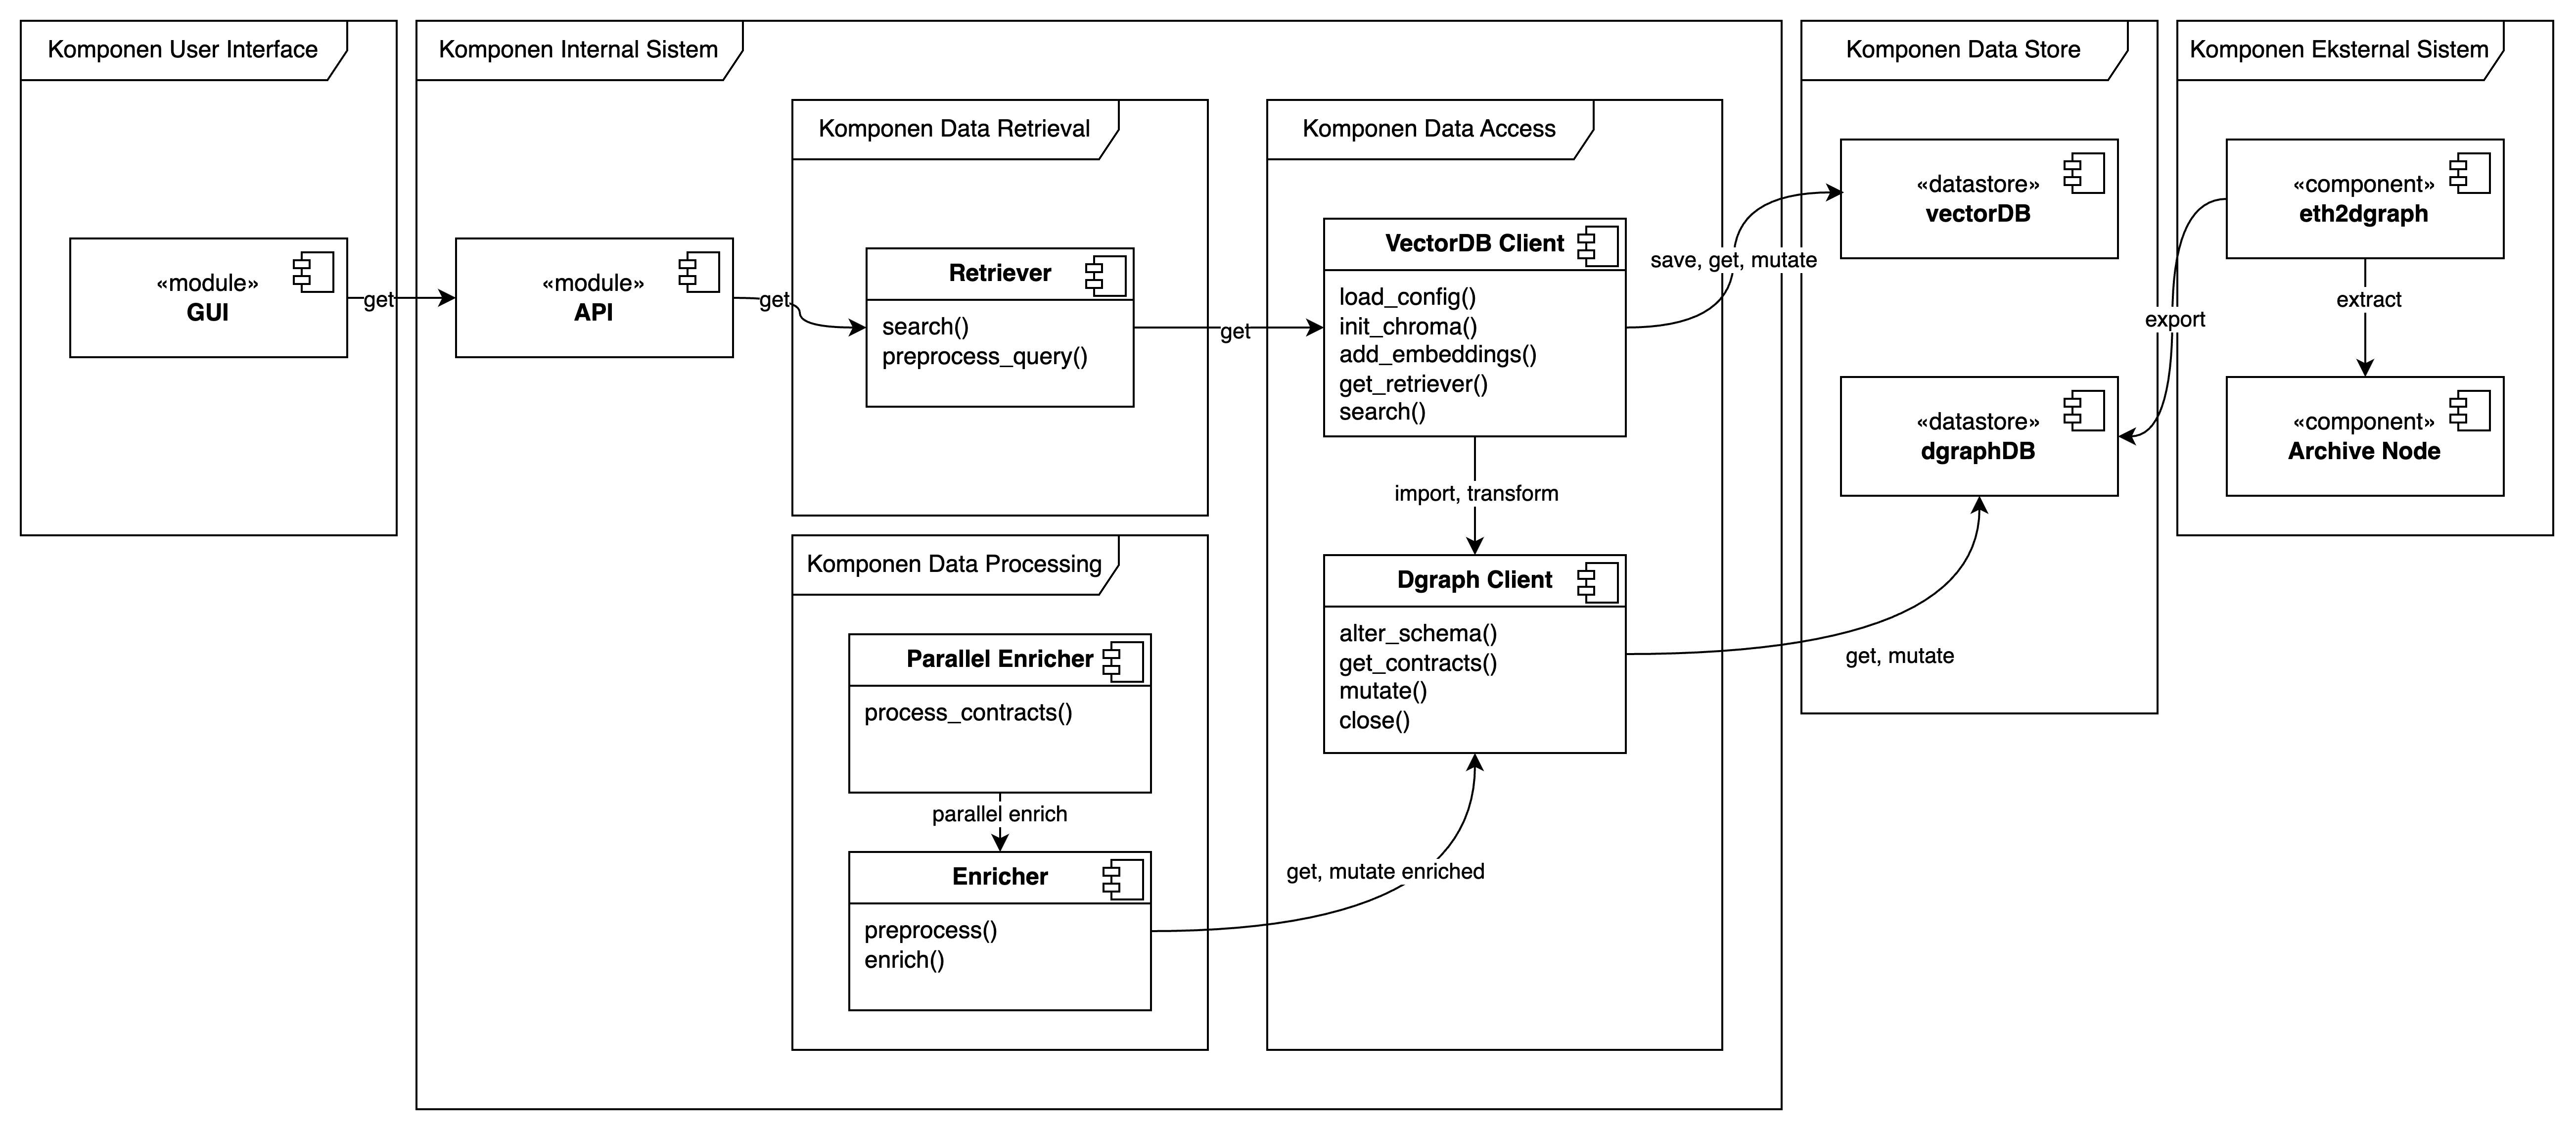
\includegraphics[width=1\textwidth]{resources/chapter-3/struktural.png}
    \caption{Rancangan struktural sistem}
    \label{image:rancangan-struktural}
\end{figure}